\documentclass[12pt]{ltjsarticle}
\usepackage{amsmath,ascmac,amssymb,mathtools,siunitx,diffcoeff,inputenc,cancel}
\usepackage{mygraphics}
\graphicspath{{../images/}}
\usepackage[backend=biber]{biblatex}
\addbibresource{../ref/ref.bib}
\usepackage[oldfont,exchangeupit]{unicommand}
\usepackage{subfiles}

%% options %%
\renewcommand{\headfont}{\bfseries}
% \numberwithin{equation}{section}
% \renewcommand*\abstractname{}
% \setlength{\parindent}{0pt}

\newcommand{\Eu}{\mathrm{eu}}
\newcommand{\Td}{\mathrm{Td}}
\newcommand{\Ch}{\mathrm{ch}}

\begin{document}
\title{指数定理まわりの勉強ノート}
\author{政岡凜太郎}
\maketitle

中原トポロジー12章の勉強の際に作ったノート。
教科書の内容はあんまり扱っていない。
TO DO: referenceをつける

\tableofcontents

\newpage
\section{Gauss-Bonnetの定理}
% いきなり指数定理を導入してもなんのこっちゃなので、
% 指数定理の中で最も古典的なGauss-Bonnetの定理から説明する。

\subsection*{不足角}
立方体の1つの頂点には、$𝜋/2$の角が3つ集まっている。
これらの角の和$3𝜋/2$を$2𝜋$から引くと$𝜋/2$が残る。
この残った角度をその頂点における不足角と呼ぶ。
不足角が$0$ならばその頂点は完全に平らであり、不足角が大きいほど頂点は尖っていると言える。
立方体は$𝜋/2$の不足角が8つの頂点それぞれにあり、その合計は$4𝜋$である。
次に、正四面体を考えてみよう。1つの頂点での不足角は$𝜋$であり、4つの頂点の合計はこの場合も$4𝜋$である。
\begin{figure}[H]
    \centering
    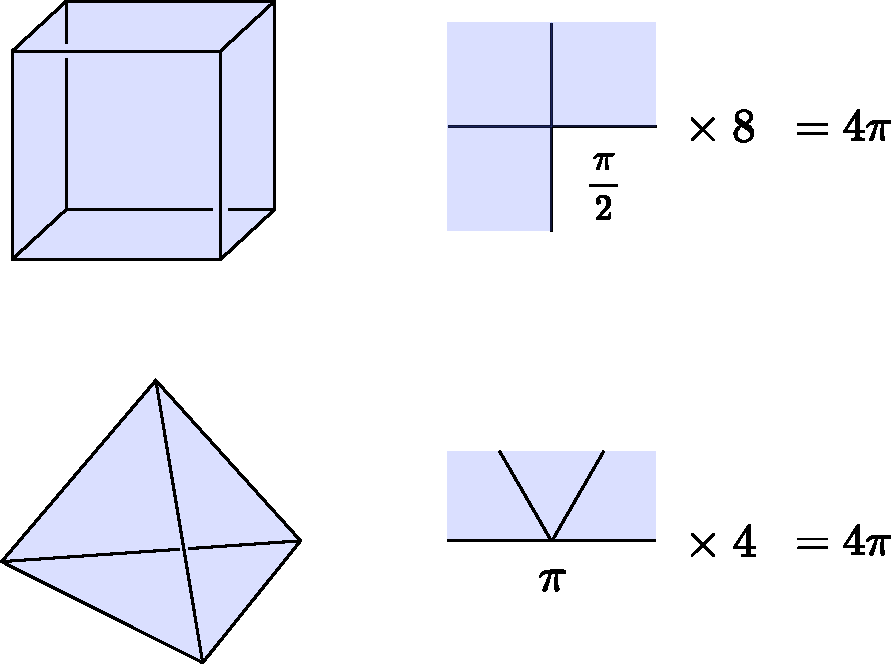
\includegraphics[width=0.5\hsize]{angulardefect}
\end{figure}
実は不足角の合計は、多面体の詳細にはよらず、種数にしかよらない。
頂点の数が$v$, 辺の数が$e$, 面の数が$f$であるような多面体を考える。
$i$番目の面が$n_i$角形だとすると、この内角の和は$𝜋(n_i-2)$であるから
\begin{align}
    (\text{不足角})
    &
    =  2𝜋v - ∑_{i=1}^f 𝜋(n_i-2) \∅
    &
    = 2𝜋v - 2𝜋e + 2𝜋f = 2𝜋χ
\end{align}
となる。ここで$∑_{i=1}^f n_i = 2e$を用いた。

Gauss-Bonnetの定理はこの式を連続的な曲面に適用できるようにしたものである。
ある曲面を多角形分割し、そのメッシュを細かくしていくと、それぞれの頂点での不足角は$0$に近づいていく。
そこで面積あたりの不足角の密度を$K$とすると、
\begin{align}
    2𝜋χ = ∫_M K 𝑑\vol 
\end{align}
と書ける。ただし$𝑑\vol$は面積要素。
これをGauss-Bonnetの定理と呼ぶ。
位相不変量が曲面上のとある量の積分で表されている、興味深い式である。
以下では不足角密度$K$を具体的に求める。

\subsection*{ホロノミー}
不足角は接ベクトルの平行移動に対するホロノミー、すなわち接ベクトルが頂点の周りを平行移動して戻ってきたたときに獲得する回転の角度とみなすことができる。
\begin{figure}[H]
    \centering
    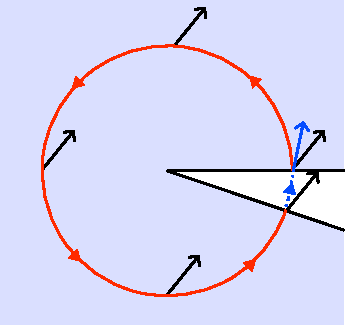
\includegraphics[width=0.4\hsize]{Holonomy}
    \caption{ホロノミー}
\end{figure}
曲面を多角形分割し、メッシュを細かくしていく極限を考える。
曲面上の領域$S$に含まれる不足角の合計はこの極限において収束し、それは$∂S$に沿って接ベクトルを平行移動したときのホロノミーによって与えられる。
注意として、ホロノミーは$2𝜋$の回転の不定性を伴うが、$S$を十分小さく取っていればこの不定性は問題にならない。

さて、ホロノミーを具体的に計算しよう。
考えている領域において$g_{ij} = δ_{ij}$となる座標をとり、曲面上の正規直交標構を$e_i$とする。
$e_i$の平行移動は共変微分
\begin{align}
    ∇_ie_j = e_kΓ_{ij}^k
\end{align}
によって与えられる。
$e_i$を正規直交標構としたので、$Γ_{ij}^k$は$j,k$について反対称となる。
また$e_i$は接空間の基底であるから、右から行列を作用させるのが自然であることに注意されよ。
% ある点の近傍において座標$(x¹, x²)$を設定し、微小な経路
% \begin{align}
%     (0, 0) → (𝑑x¹,0) → (𝑑x¹, 𝑑x²) → (0, 𝑑x²) → (0,0)
% \end{align}
% を考える。
% この経路に伴うホロノミーは、
% \begin{align}
%     e_i'
%     &
%     = e_i ℯ^{𝑑x¹∇₁}  ℯ^{𝑑x²∇₂} ℯ^{-𝑑x¹∇₁}  ℯ^{-𝑑x²∇₂} \∅
%     &
%     = e_i (1+[∇₁, ∇₂]𝑑x¹𝑑x²) \∅
%     &
%     = e_j (δ_{ji}+R_{ji12}𝑑x¹𝑑x²)
% \end{align}
% と計算される。
反対称行列($\so(2)$)を係数とする1-形式$Γ$と2-形式$ℛ$を
\begin{align}
    Γ ≔ Γ_i 𝑑x^i,␣
    (Γ)_j^k ≔ Γ_{ij}^k 𝑑x^i, ␣
    (ℛ)_{ij} ≔ ÷1{2}R_{ijkl}𝑑x^k∧𝑑x^l
\end{align}
によって定義する。
経路$∂S$に沿ったホロノミーは、
\begin{align}
    \exp(∫_{∂S}Γ) = \exp(∫_S 𝑑Γ) = \exp(∫_S ℛ)
\end{align}
と計算される。
$Γ$が反対称行列なことから$ℛ = 𝑑Γ+Γ∧Γ = 𝑑Γ$であることを用いた。
また$\SO(2)$の可換性から積分にpath orderingを付けなかった。
求めたいのは正規直交標構が回転した角度である。
\begin{align}
    ℛ = \( 0 & R_{1212} \\ -R_{1212} & 0\)𝑑x¹∧𝑑x²
\end{align}
を回転角$θ$の定義
\begin{align}
    \exp(∫_S ℛ)
    = \( \cosθ & -\sinθ \\ \sinθ & \cosθ\)
    = \exp\( 0 & -θ \\ θ & 0\)
\end{align}
と比較することで、微小な面積における不足角は
\begin{align}
    K 𝑑x¹∧𝑑x² = -R_{1212}𝑑x¹∧𝑑x² = \Pf(ℛ)
\end{align}
と求まる。ここでのPfaffianの定義は$2n$次元反対称行列に対して
\begin{align}
    \Pf(A) ≔ ÷{(-1)^n}{2^n n!}∑_{σ ∈ S_{2n}}\sign(σ)A_{σ(1)σ(2)}⋯A_{σ(2n-1)σ(2n)}
\end{align}
である。符号の付け方が通常の定義と異なることに注意。
したがって、
\begin{align}
    χ(M) = ÷1{2𝜋} ∫_M K 𝑑x¹∧𝑑x² = ÷1{2𝜋} ∫_M\Pf(ℛ) ≕ ∫_M\Eu(TM)
\end{align}
と書ける。$\Eu(TM)$はEuler形式と呼ばれる。

\subsection*{指数定理}
Gauss-Bonnetの定理を指数定理の形に整理する。
Euler標数$χ$はBetti数の交代和として表されるのだった。
\begin{align}
    χ = ∑_r (-1)^ib_r
    % = ∑_r (-1)^r \dim H_r
    = ∑_r (-1)^r \dim \ker Δ_r
\end{align}
ここで
\begin{align}
    A ≔ ⨁_{r} (𝑑_{2r}+𝑑_{2r-1}^†),␣
    A^† ≔ ⨁_{r} (𝑑_{2r-1}+𝑑_{2r}^†)
\end{align}
と定義すると、
\begin{align}
    \ind A
    &
    ≔  \dim\Ker A - \dim\Ker A^† \∅
    &
    = \dim\Ker (A^†A) - \dim\Ker (AA^†) \∅
    &
    = \dim\Ker (⨁_r Δ_{2r}) - \dim\Ker (⨁_r Δ_{2r+1}) \∅
    &
    = ∑_r (-1)^r \dim \ker Δ_r = χ
\end{align}
となる。よって
\begin{align}
    \ind A = ÷1{2𝜋} ∫_M \Pf(ℛ).
\end{align}


% \subsection*{曲面論の基本データ}
% 2次元曲面のパラメーター表示を$𝒓(u¹, u²) ∈ ℝ³$としよう。
% このパラメーター表示に沿った枠を
% \begin{align}
%     𝒆₁ ≔ ÷{∂𝒓}{∂u¹},␣
%     𝒆₂ ≔ ÷{∂𝒓}{∂u²},␣
%     𝒆₃ ≔ ÷{𝒆₁×𝒆₂}{|𝒆₁×𝒆₂|}
% \end{align}
% によって定める。
% 曲面論における第一基本量(Riemann計量) $g_{ij}$ 、
% Christoffel 記号 $Γ_{ij}^k$ 、
% 第二基本量 $h_{ij}$ は以下のように定義される。
% \begin{align}
%     𝒆_i⋅𝒆_j = g_{ij},␣
%     ∂_i𝒆_j = Γ_{ij}^k𝒆_k + h_{ij}𝒆₃.
%     % ∂_i𝒆 = -h_{ij}g^{jk}𝒆_k.
% \end{align}
% ただし$i,j$は$1,2$に値を取るとし、Einsteinの記法を用いた。
% 定義から$g_{ij}, Γ_{ij}^k, h_{ij}$は$i,j$について対称である。
% 一般相対性理論に触れたことのある読者は、$g_{ij}, Γ_{ij}^k$はお馴染みだと思われるが、$h_{ij}$には出くわさなかっただろう。
% 第二基本量$h_{ij}$は曲面を$ℝ³$にどう埋め込むかを指定する量であり、等長変換によって変わってしまうため、曲面の「内在的」な量とは言えない。
% 一般相対性理論では4次元時空をわざわざ5次元時空に埋め込んだりしないため、$h_{ij}$に対応する量は見かけなかったわけだ。

% ともかく、$g_{ij}, Γ_{ij}^k, h_{ij}$によって曲面は指定される。
% すなわち、これらが与えられれば微分方程式を解くことで元の曲面を復元することができる。
% ただし色々なconsistency conditionがあるため、これらの成分がすべて独立な自由度ではない。
% % \footnote{$Γ_{ij}^k = ÷1{2}g^{kl}(∂_ig_{jl}+∂_jg_{il}-∂_lg_{ij})$, ただし$g^{ij}$は$g_{ij}$の逆行列。}

% 以降では$g_{ij} = δ_{ij}$となるような正規直交枠を用いて議論を進める。
% ただし、このような枠は大域的には構成できるとは限らない。
% % \begin{align}
% %     𝒆_i⋅𝒆_j = δ_{ij},␣
% %     ∂_i𝒆_j = ω_{ijk} 𝒆_k + h_{ij}𝒆₃
% % \end{align}
% % \begin{align}
% %     ∇𝒆_i = 𝑑x^kω_{kij}𝒆_j = ω_{ij}𝒆_j.
% % \end{align}
% % \begin{align}
% %     ∇²𝒆 = (𝑑ω + ω∧ω)𝒆
% % \end{align}
% % $∂_i(𝒆_j⋅𝒆_k) = 0$より、$ω_{ijk}$は$j,k$に対して反対称である。
% % \begin{align}
% %     ∂_i∂_j𝒆_k = (∂_iω_{jkl} + ω_{jkm}ω_{iml}+h_{jk}h_{il})𝒆_l + ω_{jkl}h_{ik}𝒆₃
% % \end{align}

% \subsection*{Gauss曲率}
% 曲面上の曲線 $𝒓(u¹(t), u²(t))$ を考える。
% ただし$t$は曲線上を速度$1$で進むパラメータである。
% すなわち
% \begin{align}
%     |\’𝒓| = √{\’u^i\’u^j 𝒆_i ⋅ 𝒆_j } = √{g_{ij}\’u^i\’u^j} = 1
% \end{align}
% とする。
% この曲線の法曲率は
% \begin{align}
%     𝒆₃⋅\”𝒓 = \’u^i \’u^j 𝒆₃⋅∂_i∂_j𝒓 = \’u^i \’u^j 𝒆⋅∂_i𝒆_j = \’u^i\’u^j h_{ij}
% \end{align}
% によって計算される。
% 考えたい1点において$g_{ij} = δ_{ij}$とできる。
% すると拘束条件$√{δ_{ij}\’u^i\’u^j} = 1$から、法曲率の最大値$κ₁$と最小値$κ₂$はそれぞれ$h_{ij}$の最大固有値と最小固有値である。
% また$h_{ij}$が対称行列であることから、その固有ベクトルは直交する。
% つまり、ある一点を通る法曲率最大の曲線と法曲率最小の曲線は常に直交する。
% Gauss曲率を、法曲率の最大値$κ₁$と最小値$κ₂$の積によって、$K ≔ κ₁κ₂$と定義する。
% ここでの$K$の定義は等長変換で不変でない$h_{ij}$を用いていたが、実は$K$は等長変換で不変である (GaussのTheorema Egregium)。
% 実際、Riemann曲率テンソル
% \begin{align}
%     R_{ijkl} ≔ (∂_iΓ_{jk}^m -∂_jΓ_{ik}^m + Γ_{ik}^nΓ_{jn}^m - Γ_{jk}^nΓ_{in}^m )g_{ml}
% \end{align}
% を用いて$h_{ij}$を含まない形で
% \begin{align}
%     K = -÷{R_{1212}}{\det g}
% \end{align}
% と書ける。
% この証明はしないが、不足角は頂点のまわりで接ベクトルを並行移動させたときに獲得するホロノミーとみなすこともできるから、その密度が曲率テンソルで表されることはもっともである。

% \subsection*{Gauss-Bonnetの定理}

% ある一点 $𝒓(u¹, u²)$における不足角密度を計算しよう。座標変換によってこの点で$g_{ij} = δ_{ij}$かつ$h_{ij}$が対角化されていると仮定できる ($g_{ij}$を一般の座標変換で$δ_{ij}$にしたあと、直交変換で$h_{ij}$を対角化する)。
% % すると
% % \begin{align}
% %     𝒓(u¹+𝑑u¹, u²) - 𝒓(u¹,u²) = 𝒆₁𝑑u¹ + ÷1{2}∂₁𝒆₁ (𝑑u¹)² + ⋯
% % \end{align}
% % となる。
% $𝒓(u¹,u²)$の近傍において、$𝒓(u¹+n𝑑u¹,u²+m𝑑u²)$を格子点とする四角形による曲面の分割を考える。
% ただし$n, m$は整数。
% $𝒓(u¹,u²)$から周りの頂点へのベクトルを以下のように定義する。
% \begin{align}&
%     𝒂 ≔ 𝒓(u¹+𝑑u¹,u²) - 𝒓(u¹,u²) = 𝒆₁𝑑u¹+÷1{2}κ₁𝒆₃(𝑑u¹)², \\
%     &
%     𝒃 ≔ 𝒓(u¹,u²+𝑑u²) - 𝒓(u¹,u²) = 𝒆₂𝑑u²+÷1{2}κ₂𝒆₃(𝑑u²)²,\\
%     &
%     𝒄 ≔ 𝒓(u¹-𝑑u¹,u²) - 𝒓(u¹,u²) = -𝒆₁𝑑u¹+÷1{2}κ₁𝒆₃(𝑑u¹)²,\\
%     &
%     𝒅 ≔ 𝒓(u¹,u²-𝑑u²) - 𝒓(u¹,u²) = -𝒆₂𝑑u²+÷1{2}κ₂𝒆₃(𝑑u²)².
% \end{align}
% ただし微小量の2次までの寄与だけを書いている。
% 頂点$𝒓(u¹,u²)$における不足角は
% \begin{align}&
%     2π - \arccos÷{𝒂⋅𝒃}{|𝒂||𝒃|} - \arccos÷{𝒃⋅𝒄}{|𝒃||𝒄} - \arccos ÷{𝒄⋅𝒅}{|𝒄||𝒅|} - \arccos÷{𝒅⋅𝒂}{|𝒅||𝒂|} \∅
%     &
%     = 2π - 4\arccos÷{κ₁κ₂𝑑u¹𝑑u²}{4} \∅
%     &
%     = κ₁κ₂ 𝑑u¹𝑑u² = K𝑑u¹𝑑u².
% \end{align}
% 1つの頂点に割り当てられる微小面積は$𝑑u¹𝑑u²$であるから、曲面全体の不足角は
% \begin{align}
%     2πχ = ∫ K 𝑑\vol = ÷1{2} ∫ ε^{ij} ℛ_{ij}
% \end{align}
% と計算される。ここで$÷1{2}ℛ_{ij} ≔ R_{ijkl}\𝑑{x^k}∧\𝑑{x^l}$である。
% また$\det g = 1$を用いた。
% さらにこれを指数定理の形に直す。
% Euler標数$χ$はBetti数の交代和として表されるのだった。
% \begin{align}
%     χ = ∑_r (-1)^ib_r
%     % = ∑_r (-1)^r \dim H_r
%     = ∑_r (-1)^r \dim \ker Δ_r
% \end{align}
% ここで
% \begin{align}
%     A ≔ ⨁_{r} (𝑑_{2r}+𝑑_{2r-1}^†),␣
%     A^† ≔ ⨁_{r} (𝑑_{2r-1}+𝑑_{2r}^†)
% \end{align}
% と定義すると、
% \begin{align}
%     \ind A
%     &
%     =  \dim\Ker A - \dim\Ker A^† \∅
%     &
%     = \dim\Ker (A^†A) - \dim\Ker (AA^†) \∅
%     &
%     = \dim\Ker (⨁_r Δ_{2r}) - \dim\Ker (⨁_r Δ_{2r+1}) \∅
%     &
%     = ∑_r (-1)^r \dim \ker Δ_r = χ
% \end{align}
% となる。よって
% \begin{align}
%     \ind A = ÷1{4𝜋} ∫_M ε^{ij}ℛ_{ij}.
% \end{align}

\section{超対称量子力学とWitten指数}

\subsection*{Langevin方程式とFokker--Planck方程式}
超対称量子力学をとっつきやすい題材(私見)から導入することを試みる。
1次元のポテンシャル$h(x)$のもとで、粘性抵抗と、ランダムな揺動$η$によって運動する粒子を考える。
この粒子は以下の運動方程式に従う。
\begin{align}
    m÷{𝑑x²}{𝑑t²} = -γ÷{𝑑x}{𝑑t} -÷{∂h}{∂x} + η(t)
\end{align}
粘性抵抗が十分大きい場合には2階微分項を落として
\begin{align}
   ÷{𝑑x}{𝑑t} = -÷{𝑑h}{𝑑x} + η(t)
\end{align}
としてよい。簡単のため物理定数は全て$1$とした。
この確率微分方程式を考える。
ここで、$η(t)$は白色ノイズとする。$η(t)$についての平均は
\begin{align}&
   ⟨X⟩_η = ÷1{𝒵_η} ∫\𝒟{η} X \exp(-÷{β}{4} ∫\𝑑{t} η(t)²), \\
   &
   𝒵_η =  ∫\𝒟{η}\exp(-÷{β}{4} ∫\𝑑{t} η(t)²).
\end{align}
によって与える。
等価な系の記述として、粒子の軌跡を追いかけるのではなく、確率分布$P(x,t)$の時間発展を考えることもできる。その場合、$P(x,t)$は以下のFokker--Planck方程式に従う。
\begin{align}
    ÷{∂}{∂t}P(x,t) = ÷{∂}{∂x}(÷1{β}÷{∂}{∂x}+÷{∂h}{∂x})P(x,t).
\end{align}
導出は付録を参照。
Fokker--Planck方程式の固定点は
\begin{align}
    P_{eq}(x) ≔ ÷{ℯ^{-βh(x)}}{𝒵},␣ 𝒵 = ∫\𝑑{x} ℯ^{-βh(x)}
\end{align}
で与えられる。

\subsection*{超対称量子力学}
以下では式の見やすさのために、$h(x) → 2h(x)/β$, $t → βt$と置き換える。
つまりFokker--Planck方程式を
\begin{align}
    ÷{∂P}{∂t} = ÷{∂}{∂x}(÷{∂}{∂x} + 2÷{𝑑h}{𝑑x})P(x,t)
\end{align}
とする。
これを解くためには右辺の演算子についての固有ベクトルを求めればよい。
実はこの演算子のスペクトルは非負になる。
これを示すために相似変換
\begin{align}
    P(x,t) ↦ ψ(x,t) ≔ ℯ^{h(x)}P(x,t)
\end{align}
を考えよう。$ψ(x,t)$が従う方程式は
\begin{align}
    ÷{∂ψ}{∂t}
    &
    = ℯ^{h(x)}÷{∂}{∂x}(÷{∂}{∂x}+2÷{𝑑h}{𝑑x})ℯ^{-h(x)}ψ(x) \∅
    &
    = (÷{∂}{∂x}-÷{𝑑h}{𝑑x})(÷{∂}{∂x}+÷{𝑑h}{𝑑x})ψ(x).
\end{align}
で与えられる。
この式は虚時間Schrödinger方程式
\begin{align}
    ÷{∂ψ}{∂t} = -H₊ψ,␣ H₊ = (÷{∂}{∂x}-÷{𝑑h}{𝑑x})(-÷{∂}{∂x}-÷{𝑑h}{𝑑x})
\end{align}
とみなせる。
$H₊$は半正定値なのでFokker--Planck方程式のスペクトルは非負になる。
基底状態は
\begin{align}
    ψ_{eq}(x) = √{𝒵}ℯ^{h(x)} P_{eq}(x) = ÷{ℯ^{-h(x)}}{√{𝒵}}
\end{align}
で与えられる。

さて、ここまででFokker--Planck方程式と等価な量子系を得たわけだが、この量子系は超対称量子力学と深く関係している。
これを見るために$h(x)$を$-h(x)$に置き換えたHamiltonian
\begin{align}
    H₋ ≔  (÷{∂}{∂x}+÷{𝑑h}{𝑑x})(-÷{∂}{∂x}+÷{𝑑h}{𝑑x})
\end{align}
を考えてみる。
$H₊$と$H₋$は以下のように書くことができる。
% $ψ(x,t)$が満たす方程式をFokker--Planck方程式から導くと、
% \begin{align}
%     ÷{∂}{∂t}ψ(x,t)
%     &
%     = -(-¡÷{∂}{∂x}+¡÷{𝑑h}{𝑑x})(-¡÷{∂}{∂x}-¡÷{𝑑h}{𝑑x})ψ(x, t)
%     ≕ -H₊ψ(x,t)
% \end{align}
% となる。
% \begin{align}
%     ÷{∂}{∂t}ψ(x,t)
%     = -(-¡÷{∂}{∂x}-¡÷{𝑑h}{𝑑x})(-¡÷{∂}{∂x}+¡÷{𝑑h}{𝑑x})ψ(x, t)
%     ≕ -H₋ψ(x,t)
% \end{align}
\begin{align}
    H₊ ≔ A^†A,␣H₋ ≔ AA^†,␣
    A = -¡(÷{𝑑}{𝑑x}+÷{𝑑h}{𝑑x}).
\end{align}
% Hamiltonian $H₊$はポテンシャル$h(x)$の下でのFokker--Planck方程式を与え、
% $H₋$は$-h(x)$の下でのFokker--Planck方程式を与える。
注目するべきは、$H₋$がゼロモードを除いて、$H₊$と同じスペクトルをもつことである。
実際、$H₊$の固有値$E_n$の固有ベクトル$|E_n⟩$に対して、$A|E_n⟩$は同じ固有値をもつ$H₋$の固有ベクトルになる:
\begin{align}
    H₋A|E_n⟩ = AA^†A|E_n⟩ = AH₊|E_n⟩ = E_nA|E_n⟩.
\end{align}
このような固有状態のペアができないのは$A|E_n⟩ = 0$の場合。
すなわち$A^†A|E_n⟩ = H₊|E_n⟩ = 0$の場合である。
% また、
% \begin{align}
%     Aℯ^{-H₊t} = ℯ^{-H₋t}A,␣
%     A^†ℯ^{-H₋t} = ℯ^{-H₊t}A^†
% \end{align}
% であるから、$H₊$による虚時間発展を$H₋$による虚時間発展にマップできる(逆も然り)。
% ただしゼロモードについては対応関係はない。
% もとの確率過程の言葉で言うと、
% \begin{align}&
%     (-¡÷{∂}{∂x}-2¡÷{𝑑h}{𝑑x})\exp(t÷{∂}{∂x}(÷1{2}÷{∂}{∂x}+÷{𝑑h}{𝑑x})t) \∅
%     &
%     = \exp(t÷{∂}{∂x}(÷1{2}÷{∂}{∂x}-÷{𝑑h}{𝑑x}))(-¡÷{∂}{∂x}-2¡÷{𝑑h}{𝑑x})
% \end{align}

$H₊$と$H₋$は超対称パートナーと呼ばれ、超対称量子力学を用いることで整理される。
まず、Hilbert空間がbosonicな部分空間とfermionicな部分空間の直和として
\begin{align}
    ℋ = ℋ_𝐵 ⊕ ℋ_𝐹
\end{align}
と書かれているとしよう。波動関数はbosonicな成分とfermionicな成分によって
\begin{align}
    Ψ(x) = \( ψ_𝐵(x) \\ ψ_𝐹(x)\)
\end{align}
と表される。
ここで複素超電荷$𝒬, 𝒬^†$を以下のように定義する。
\begin{align}
    𝒬 ≔ \( 0&0\\√2A&0\),␣
    𝒬^† ≔ \( 0&√2A^†\\0&0\).
\end{align}
これらは冪零性$𝒬² = 𝒬^{†2} = 0$を満たす。
またHamiltonianを以下のように定義する。
\begin{align}
    H = ÷1{2}\{𝒬, 𝒬^†\} = \( A^†A & 0\\0& AA^†\) = \( H₊&0\\0&H₋\)
\end{align}
Hamiltonian $H$によって定められる模型をWitten模型と呼ぶ。
また模型を定めるポテンシャル$h(x)$は超ポテンシャルと呼ばれる。

この模型がもつ超対称性は演算子の間の代数的な関係式としてまとめることができる。
まずHamiltonianは以下の交換関係を満たす。
\begin{align}
    [H, 𝒬] = [H, 𝒬^†] = 0.
\end{align}
これらの式は$𝒬, 𝒬^†$が$H$の固有値を変えないことを意味する。
次に
\begin{align}
    (-1)^F ≔ \( 1&0\\0&-1\)
\end{align}
と定義する。この演算子は$((-1)^F)² = 1$および$[H, (-1)^F] = 0$を満たす。
したがって任意のエネルギー固有状態は$(-1)^F$の固有値が$+1$の状態(boson)と$-1$の状態(fermion)に分かれる。
また$\{(-1)^F,𝒬\} = \{(-1)^F,𝒬^†\}=0$から、$𝒬, 𝒬^†$は$(-1)^F$の固有値を反転する。
以上で述べた演算子の間の関係式を超対称性関係と呼ぶ。
改めてまとめると、以下のようになる。
% また$[H₊, (-1)^F] = [H₋, (-1)^F] = 0$である。
\begin{align}&
    𝒬² = 𝒬^{†2} = 0 \\
    &
    \{𝒬, 𝒬^†\} = 2H \\
    &
    [H, 𝒬] = [H, 𝒬^†] = 0 \\
    &
    ((-1)^F)² = 1 \\
    &
    [H, (-1)^F] = 0 \\
    &
    \{(-1)^F, 𝒬\} = \{(-1)^F, 𝒬^†\} = 0
\end{align}
ただし$𝒬, 𝒬^†, H, (-1)^F$は独立なものではなく、
\begin{align}
    ÷1{2}[𝒬^†, 𝒬] = (-1)^FH 
\end{align}
が成り立つ。
また複素超電荷$𝒬, 𝒬^†$の代わりに実超電荷$Q ≔ ÷1{√2}(𝒬 + 𝒬^†)$を用いることもできる。この場合、超対称性関係は
\begin{align}&
    H = Q² \\
    &
    \{(-1)^F, Q\} = 0 \\
    &
    ((-1)^F)² = 0
\end{align}
となる。

bosonicな状態とfermionicな状態の間の対応は超対称性関係だけから導くことができる。
まず$((-1)^F)² = 0,~[H, (-1)^F] = 0$から任意の固有状態はbosonicまたはfermionicである。
エネルギー$E > 0$をもつ規格化されたbosonicな固有状態$|b_E⟩$に対し、
\begin{align}&
    H𝒬|b_E⟩ = 𝒬H|b_E⟩ = E𝒬|b_E⟩,\\
    &
    (-1)^F𝒬|b_E⟩ = -𝒬(-1)^F|b_E⟩ = -𝒬|b_E⟩
\end{align}
より$𝒬|b_E⟩$はエネルギー$E$のfermionicな固有状態である。
また、この状態のノルムは
\begin{align}
    ⟨b_E|𝒬^† 𝒬|b_E⟩
    &
    = ÷1{2}⟨b_E|\{𝒬^†,𝒬\}|b_E⟩-÷1{2}⟨b_E|[𝒬^†,𝒬]|b_E⟩ \∅
    &
    = ⟨b_E|H|b_E⟩ + ⟨b_E|(-1)^FH|b_E⟩ \∅
    &
    = 2E
\end{align}
で与えられる。したがって、
\begin{align}
    |f_E⟩ = ÷1{√{2E}}𝒬|b_E⟩
\end{align}
とおける。同様に、規格化されたfermionicな固有状態$|f_E⟩$が与えられれば、
\begin{align}
    |b_E⟩ = ÷1{√{2E}}𝒬^†|f_E⟩
\end{align}
によってbosonicな固有状態が構成される。



\subsection*{Witten指数}
Witten指数を以下のように定義する。
\begin{align}
    \ind ≔ \dim \Ker H₊ - \dim \Ker H₋ = \dim \Ker A - \dim \Ker A^† .
\end{align}
$H₊$と$H₋$のスペクトルはゼロモードを除いて等しいという事実から、Witten指数は以下のように定義することもできる。
\begin{align}
    \ind = \Tr (-1)^F.
\end{align}
ただし、この表示において単純に
\begin{align}
    \Tr(-1)^F = \Tr\( 1&0\\0&-1\) = 0
\end{align}
とはできない。
なぜならばそれぞれのブロックの$1$は無限次元のHilbert空間に作用する恒等演算子であり、指数の定義は$∞-∞$の形になっているからである。
実際には、指数の定義は以下のように正則化(熱核正則化)した形で理解するべきである。
\begin{align}
    \ind = \Tr[(-1)^F ℯ^{-βH}]
    = \Trℯ^{-βH₊} - \Trℯ^{-βH₋} ,␣ β > 0.
\end{align}
この$β$はFokker--Planck方程式における$β$とは全く別物なので注意。
別の正則化として、固有値にカットオフ$Λ$を定めるというものもある。この場合、
\begin{align}
    \ind = ∑_{\substack{λ₊ ∈ \Spec H₊ \\ λ₊ ≤ Λ}} 1 - ∑_{\substack{λ₋ ∈ \Spec H₋ \\ λ₋ ≤ Λ}} 1
\end{align}
となる。
ただし、連続スペクトルがある場合には正則化に依存する補正項が入ることがあるため注意が必要である(付録を参照)。
% このようなカーネルを用いた指数の定義において、Hilbert空間が無限次元であることが本質的である。
% $A$がもし有限次元ならば、$AA^†$と$A^†A$は同じ数のゼロモードを持ってしまい、$\ind = 0$となる。

次にWitten指数の幾何学的解釈を与えよう。
実は、Witten指数は
\begin{align}
    \ind = (\text{$h(x)$の極小点の数}) - (\text{$h(x)$の極大点の数})
    \label{Witten index from Morse theory}
\end{align}
として計算できる。
この等式の導出は後ほど。
右辺は$h(x)$の連続的な変形に対して常に保たれるため、位相不変量と言える。

例えば$h(x)$が$x → ±∞$で正の無限大に発散する場合を考えよう。
この時ポテンシャル$h(x)$で指定されるFokker--Planck方程式には一意な熱平衡状態($=$ゼロモード)が存在するが、
$-h(x)$の下では粒子が$x → ±∞$に逃げていくので熱平衡状態は存在しない。
したがってWitten指数は$1-0 = 1$になる。
一方で$h(x)$の極小点の数は極大点の数より必ず$1$大きくなる。

また$x ∈ S¹$とすることもできる。この時$h(x)$が有限なポテンシャルならば、$±h(x)$に対して一意な熱平衡状態が存在する。よってWitten指数は$1-1=0$である。
一方$h(x)$の極大点の数と極小点の数は一致する。

\subsection*{調和振動子}
具体例として、$h(x) = x²/2$の場合を考えてみる。
この時
\begin{align}
    A = -¡(÷{𝑑}{𝑑x} + ÷{𝑑h}{𝑑x}) = -¡(÷{𝑑}{𝑑x}+x) = -√{2}¡ a
\end{align}
である。ここで$a$は調和振動子の消滅演算子である。
Hamiltonianは
\begin{align}
    H = \( A^†A & 0 \\ 0 & AA^†\) = 2\( a^†a & 0 \\ 0& aa^†\)
\end{align}
となる。 
ゼロモードはbosonicなセクターのみに存在し、
\begin{align}
    Ψ(x) = ℯ^{-x²/2}|0⟩
\end{align}
で与えられる。ここで$|0⟩$はfermionに対するFock真空である。
Witten指数は
\begin{align}
    \ind = \dim\Ker a - \dim\Ker a^† = 1-0 = 1
\end{align}
である。
また$h(x) = x²/2$の極小点は$1$個、極大点は$0$個であり、幾何学的な指数の定義(\ref{Witten index from Morse theory})が成り立っていることが分かる。

次に$h(x) = -x²/2$の場合を考える。このとき
\begin{align}
    H = 2\( aa^† & 0 \\ 0 & aa^† \)
\end{align}
であり、先ほどとは逆でfermionicなセクターが以下のゼロモードをもつ。
\begin{align}
    Ψ(x) = ℯ^{-x²/2}ψ^†|0⟩
\end{align}
ただし$ψ^†$はfermionの生成演算子である。
Witten指数は
\begin{align}
    \ind = \dim\Ker a^† - \dim\Ker a = 0-1 = -1
\end{align}
となる。

% 生成消滅演算子が非自明な指数を持つことは、Hermitianな位相演算子が定義できないことと関係している。
% \begin{align}
%     a = ℯ^{¡φ}√N
% \end{align}
% によって位相演算子$φ$を定義する。
% ここで$N$は粒子数演算子である。
% もし$ℯ^{¡φ}$がユニタリ($φ$がHermitian)ならば、
% \begin{align}
%     a^†a = N,␣ aa^† = ℯ^{¡φ}N(ℯ^{¡φ})^†
% \end{align}
% となり、$a^†a$と$aa^†$はユニタリ同値になる。
% これは$\ind = 0$を意味する。



\section{Morse理論}

\subsection*{微分形式の超対称量子力学による表現}
% \begin{align}
%     c^i ≔ g^{ij}(x)c_j,␣ c^†_i ≔ g_{ij}(x)c^{†j}.
% \end{align}
この節ではより一般的な形で$d$次元Riemann多様体$M$上の超対称量子力学を考える。
まず複素超電荷として、以下の演算子を考える。
% \begin{align}&
%     𝒬 ≔ (p^†_i - ¡÷{∂h}{∂x^i})ψ^{†i},␣
%     𝒬^† ≔ (p_i + ¡÷{∂h}{∂x^i})ψ^i.
% \end{align}
\begin{align}&
    𝒬 ≔ ψ^{†i}(p_i - ¡÷{∂h}{∂x^i}),␣
    𝒬^† ≔ ψ^i(p^†_i + ¡÷{∂h}{∂x^i}).
\end{align}
$p_i$は運動量演算子であり、交換関係
\begin{align}
    [p_i, f(x)] =  -¡∂_if(x)
\end{align}
に従う。
一般の多様体上の量子力学では$p_i^† = p_i$とはできないことに注意する。
微分形式の文脈で外微分の随伴$𝑑^†$が計量$g_{ij}$およびその行列式$\det g$による寄与を含むことを思い出されよ。
また$ψ^i$はフェルミオン演算子であり、
% \begin{align}
%     [p_i, ψ^j] = 0,␣ [p_i, ψ^†_j] = 0,␣
%     \{ψ^{†i}, ψ^j\} = δ^i_j
% \end{align}
\begin{align}&
    [p_i, ψ_j] = 0,␣ [p_i, ψ^{†j}] = 0, \\
    &
    \{ψ_i,ψ_j\}=\{ψ^{†i},ψ^{†j}\}=0,␣
    \{ψ^{†i}, ψ^j\} = δ^i_j
\end{align}
に従うとする。
この定義には流儀がありそうで、$[p_i,ψ^j] = 0, [p_i, ψ^†_j] = 0$としている文献もあった。
微分形式との対応関係を尊重してこのような定義にしている。
$𝒬$の冪零性は以下のように確認される。
\begin{align}
    𝒬²
    = ψ^{†i}ψ^{†j}(p_i - ¡÷{∂h}{∂x^i})(p_j - ¡÷{∂h}{∂x^j}) 
    = 0.
\end{align}
$𝒬^†$についても同様。
ここで、fermionの生成消滅演算子は形式的に
\begin{align}
    ψ^{†j} = 𝑑x^j∧,␣
    ψ_j = ι_{∂_j}
\end{align}
と置き換えることができる。
このように見ると、波動関数と微分形式の間に
\begin{align}
    Ψ_{i₁⋯i_p}(x)ψ^{†i₁}⋯ψ^{†i_p}|0⟩
    ↔
    Ψ_{i₁⋯i_p}(x)𝑑x^{i₁}∧⋯∧𝑑x^{i_p}
\end{align}
という対応がつく。
また内部積$ι_{∂_j}$は
\begin{align}
    ι_{∂_j}(𝑑x^{i₁}∧⋯∧𝑑x^{i_p})
    = ∑_n (-1)^{n-1} δ^{i_n}_j𝑑x^{i₁}∧⋯∧\cancel{𝑑x^{i_n}} ∧⋯∧𝑑x^{i_p}
\end{align}
を線形に拡張して得られるが、これは$ψ_j$の作用に完全に対応している。
したがって、fermionは微分形式の自由度を表しているとみなすことができ、$n$-fermion状態は$n$-formに対応する。

\subsection*{共変微分}
この節の内容は超対称量子力学のHamilton形式をすっきりまとめるためのものであるが、次節のWitten指数の計算ではそこまで必要ではない。
曲がった多様体上では偏微分に対応する演算子$p_i$は使いにくいため、
共変微分に対応する演算子
% \begin{align}
%     π_i ≔ p_i - ¡ Γ_{ij}^k ψ^†_k ψ^j
% \end{align}
\begin{align}
    π_i ≔ p_i + ¡ Γ_{ij}^k ψ^{†j}ψ_k = -¡∇_i
\end{align}
を定義する。$Γ_{ij}^k$はLevi-Civita接続
\begin{align}
    Γ_{ij}^k = ÷1{2} g^{kl}(∂_ig_{jl}+∂_jg_{il}-∂_lg_{ij})
\end{align}
である。この演算子は
\begin{align}&
    [π_i, ψ_j] = -¡Γ_{ij}^kψ_k,␣
    [π_i, ψ^j] = ¡Γ_{ik}^jψ^k, \\
    &
    [π_i, ψ^†_j] = -¡Γ_{ij}^kψ^†_k, ␣
    [π_i, ψ^{†j}] = ¡Γ_{ik}^jψ^{†k}, \\
    &
    [π_i, π_j] = R_{ijkl}ψ^{†k}ψ^l
\end{align}
を満たす。ここで$R_{ijkl}$はRiemannテンソル
\begin{align}
    R_{ijkl} ≔ (∂_iΓ_{jk}^m-∂_jΓ_{ik}^m+Γ_{ik}^nΓ_{jm}^k - Γ_{jk}^nΓ_{im}^k) g_{ml}
\end{align}
である。また$π_i$の共役は以下のように書かれる。
% \begin{align}&
%     [π_i-π_i^†, f(x)] = 0,
%     [π_i-π_i^†, ψ_j^†] = 0
% \end{align}
\begin{align}
    π_i^† = π_i - ¡÷1{√{\det g}}∂_i√{\det g} = π_i - ¡Γ_{ij}^j.
\end{align}
特に$g_{ij} = δ_{ij}$としたとき、$π_i$はHermitianになる。
超電荷$𝒬, 𝒬^†$を定義する際に、$p_i$の代わりに$π_i$を用いて
% \begin{align}
%     𝒬 = (π_i - ¡÷{∂h}{∂x^i})ψ^{†i},␣
%     𝒬^† = (π_i + ¡÷{∂h}{∂x^i})ψ^i
% \end{align}
\begin{align}&
    𝒬 ≔ ψ^{†i}(p_i - ¡÷{∂h}{∂x^i})= ψ^{†i}(π_i - ¡÷{∂h}{∂x^i}), \\
    &
    𝒬^† ≔ ψ^i(p^†_i + ¡÷{∂h}{∂x^i})= ψ^i(π_i + ¡÷{∂h}{∂x^i})
\end{align}
と表せる。
% $𝒬^†$の表示は
% \begin{align}
%     π_iψ^i = (p_i - ¡Γ_{ij}^kψ^†_kψ^j)ψ^i = p_iψ^i
% \end{align}
$𝒬$の表示は
\begin{align}
    ψ^{†i}π_i = ψ^{†i}(p_i + ¡Γ_{ij}^kψ^{†j}ψ_k) = ψ^{†i}p_i
\end{align}
より分かる。
% $𝒬$の表示は
% \begin{align}
%     π_iψ^{†i}
%     = ψ^{†i}π_i + ¡Γ_{ij}^iψ^{†j}
%     = ψ^{†i}π^†_i
% \end{align}
$𝒬^†$の表示は
\begin{align}
    ψ^iπ_i
    = π_iψ^i - [π_i,ψ^i]
    = π_iψ^i - ¡Γ_{ij}^iψ^j
    = π_i^†ψ^i
\end{align}
より分かる。
% \begin{align}&
%     [(π_i-p^†_i)ψ^{†i}, ψ^j] \∅
%     &
%     = (π_l-p^†_l)g^{lj} - ¡Γ_{ik}^jψ^kψ^{†i} - ¡∂_ig^{jk}ψ_kψ^{†i} \∅
%     &
%     = -¡Γ_{li}^kg^{lj}ψ^†_kψ^i-¡Γ_{il}^jg^{kl}ψ_kψ^{†i} - ¡∂_ig^{jk}ψ_kψ^{†i} 
% \end{align}
% $𝒬$の表示は
% \begin{align}
%     ψ^{†i}π_i = ψ^{†i}(p_i + ¡Γ_{ij}^kψ^{†j}ψ_k) = ψ^{†i}p_i
% \end{align}
% より分かる。
% $𝒬^†$の表示は一目見ただけでは分からないかもしれないが、$𝒬^†$が座標の取り方によらないことから、局所的に平坦な座標で確かめれば良い。
% このとき
% \begin{align}
%     𝒬^† = (p_i+¡÷{∂h}{∂x^i})ψ^i = ψ^i(p_i+¡÷{∂h}{∂x^i})
% \end{align}
% であり、あとは一般の座標に拡張すればよい。
Hamiltonは以下のように計算される。
% \begin{align}
%     2H 
%     &
%     = \{𝒬, 𝒬^†\}  \∅
%     &
%     = {(π_i-¡÷{∂h}{∂x^i})ψ^{†i},(π_j+¡÷{∂h}{∂x^j})ψ^j} \∅
%     &
%     = \{π_iψ^{†i},π_jψ^j\}+\{ψ^{†i},ψ^j\}÷{∂h}{∂x^i}÷{∂h}{∂x^j} \∅
%     &␣
%     + ¡{π_iψ^{†i},÷{∂h}{∂x^j}ψ^j}
%     - ¡{π_jψ^j,÷{∂h}{∂x^i}ψ^{†i}}  \∅
%     &
%     = Δ+g^{ij}÷{∂h}{∂x^i}÷{∂h}{∂x^j} 
%     - ¡[π_i,÷{∂h}{∂x^j}ψ^j]ψ^{†i}
%     + ¡[π_j,÷{∂h}{∂x^i}ψ^{†i}]ψ^j  \∅
%     &
%     = Δ+g^{ij}÷{∂h}{∂x^i}÷{∂h}{∂x^j}
%     +(÷{∂²h}{∂x^i∂x^j}-Γ_{ij}^k÷{∂h}{∂x^k})[ψ^{†i},ψ^j].
% \end{align}
\begin{align}
    2H 
    &
    = \{𝒬, 𝒬^†\}  \∅
    &
    = {ψ^{†i}(π_i-¡÷{∂h}{∂x^i}),ψ^j(π_j+¡÷{∂h}{∂x^j})} \∅
    &
    = \{ψ^{†i}π_i,ψ^jπ_j\}+\{ψ^{†i},ψ^j\}÷{∂h}{∂x^i}÷{∂h}{∂x^j} \∅
    &␣
    + ¡ψ^{†i}[π_i,ψ^j÷{∂h}{∂x^j}]-¡ψ^j[π_j,ψ^{†i}÷{∂h}{∂x^i}] \∅
    &
    = Δ+g^{ij}÷{∂h}{∂x^i}÷{∂h}{∂x^j}+[ψ^{†i},ψ^j](÷{∂²h}{∂x^i∂x^j} - Γ_{ij}^k÷{∂h}{∂x^k}).
\end{align}
ここで$Δ$は以下のように成分表示される。
% \begin{align}
%     Δ &≔ \{π_iψ^{†i},π_jψ^j\} \∅
%     &
%     = π_i[ψ^{†i},π_j]ψ^j
%     + [π_i,π_j]ψ^{†i}ψ^j
%     + π_jπ_i\{ψ^{†i}, ψ^j\} 
%     -π_j[π_i,ψ^j]ψ^{†i} \∅
%      &
%     = g^{ij}(π_iπ_j + ¡Γ_{ij}^kπ_k) - R_{ijkl}ψ^{†i}ψ^jψ^{†k}ψ^l
% \end{align}
\begin{align}
    Δ &≔ \{𝑑,𝑑^†\} = \{ψ^{†i}π_i,ψ^jπ_j\} \∅
    &
    = ψ^{†i}[π_i,ψ^j]π_j
    +ψ^{†i}ψ^j[π_i,π_j]
    +\{ψ^{†i},ψ^j\}π_jπ_i
    -ψ^j[ψ^{†i},π_j]π_i \∅
     &
    = g^{ij}(π_iπ_j + ¡Γ_{ij}^kπ_k) + R_{ijkl}ψ^{†i}ψ^jψ^{†k}ψ^l
\end{align}
である。ただし公式
% \begin{align}
%     \{AB,CD\} = A[B,C]D+[A,C]BD+CA\{B,D\} - C[A,D]B
% \end{align}
\begin{align}
    \{AB,CD\} = A[B,C]D+AC[B,D]+\{A,C\}DB - C[A,D]B
\end{align}
を用いた。
さらに、等式$R_{ijkl}+R_{iklj}+R_{iljk}=0$および$R_{ijkl}=-R_{ijlk}$から
\begin{align}
    R_{ijkl}ψ^{†i}ψ^{†j}ψ^kψ^l
    &
    = (-R_{iklj}-R_{iljk})ψ^{†i}ψ^{†j}ψ^kψ^l \∅
    &
    = (R_{ikjl}-R_{iljk})ψ^{†i}ψ^{†j}ψ^kψ^l \∅
    &
    = -2R_{ijkl}ψ^{†i}ψ^jψ^{†k}ψ^l
    + 2R_{ikjl}g^{kj}ψ^{†i}ψ^l \∅
    &
    = -2R_{ijkl}ψ^{†i}ψ^jψ^{†k}ψ^l
    - 2R_{ij}ψ^{†i}ψ^j
\end{align}
となる。よって、
\begin{align}
    Δ = g^{ij}(π_iπ_j + ¡Γ_{ij}^kπ_k) - R_{ij}ψ^{†i}ψ^j - ÷1{2}R_{ijkl}ψ^{†i}ψ^{†j}ψ^kψ^l
\end{align}
となる。Laplacianのこのような成分表示は微分形式の理論においてWeitzenböck identityとして知られている。

\subsection*{Morse理論}
さて、Hamiltonian $H = ÷1{2}\{𝒬,𝒬^†\}$で定められる超対称量子力学系に対し、Witten指数を求めよう。
$(-1)^F$はfermion数が偶数個の状態に対して固有値$+1$を、奇数個の状態に対して固有値$-1$を与える演算子として定義される。
よってWitten指数は
\begin{align}
    \ind = (\text{偶数fermionのゼロモードの数}) - (\text{奇数fermionのゼロモードの数})
\end{align}
となる。
超電荷$𝒬, 𝒬^†$は
\begin{align}&
    𝒬 = ℯ^{-h}(-¡ψ^{†i}∂_i)ℯ^{h} = -¡ℯ^{-h}𝑑ℯ^{h},\\
    &
    𝒬^† = ℯ^{h}(-¡ψ^i∂_i)ℯ^{-h} = -¡ℯ^{h}𝑑^†ℯ^{-h}
\end{align}
と書き直せる。
考えている多様体$M$がコンパクトで$h(x)$が有限の場合、
Witten指数は$h(x)$の連続変形に対して不変なので、
特に$h(x)=0$の場合を考えることができる。
このとき$𝒬 = 𝑑, 𝒬^† = 𝑑^†, H = ÷1{2}Δ$であり、ゼロモードは調和形式である。
したがって、Witten指数はEuler数になる。
\begin{align}
    \ind = \Tr (-1)^F = ∑_r (-1)^rb_r = χ.
\end{align}


次に、Witten指数の幾何学的解釈(\ref{Witten index from Morse theory})を導出しよう。多様体上に関数$h(x)$を考え、その極値から多様体の情報を引き出す枠組みはMorse理論とよばれる。超対称量子力学によってMorse理論は物理的考察から理解することができる。
Witten指数が位相不変量であることから、$h(x)$を$h(x)/ħ$で置き換えて$ħ → 0$の極限を取ってよい。
このとき$∂_ih(x) ≠ 0$であるような点においてポテンシャルが発散するため、ゼロモードは$h(x)$の臨界点付近に局在する。
臨界点とは、$h(x)$が極値をとる点$x$のことである。
臨界点$x₀ ∈ M$においてHessian $∇_i∇_jh = ∂_i∂_jh$を対角化する座標をとると、
\begin{align}
    h(x) ≈ ∑_i ÷{λ_i}{2} (x^i-x₀^i)²
\end{align}
と表せる。ここで$λ_i$はHessianの固有値である。
臨界点付近に局在するモードに対するHamiltonianは
\begin{align}&
    H ≈ ∑_i ÷1{ħ²}\( A_i^†A_i & 0 \\ 0 & A_iA_i^†\),
    ␣
    A_i ≔ -¡ħ÷{∂}{∂x^i} - ¡λ_i(x^i-x₀^i)
    % H_i = -÷{ħ²}{2}÷{∂²}{{∂x^i}^2}+ ÷1{2}λ_i²(x^i-x₀^i)² + ÷1{2}ħλ_iσ^z
\end{align}
と近似できる。
各座標軸に対応する項は調和振動子の超対称量子力学系であり、$λ_i > 0$の場合はbosonicなゼロモード
\begin{align}
    \exp(-÷{λ_i}{2ħ}(x^i-x₀^i)²)|0⟩,
\end{align}
$λ_i < 0$の場合はfermionicなゼロモード
\begin{align}
    \exp(÷{λ_i}{2ħ}(x^i-x₀^i)²)ψ^{†i}|0⟩
\end{align}
がある。 Hessianの負の固有値が$r$個あるとき、その臨界点のMorse指数は$r$であるという。
臨界点$x₀$付近に存在するゼロモードはfermion数が$r$となる以下のゼロモードをもつ。
\begin{align}
    \exp(-∑_i÷{|λ_i|}{2ħ}(x^i-x₀^i)²) ψ^{†i₁}⋯ψ^{†i_r}|0⟩
\end{align}
ここで$i₁,…,i_r$はHessianの負の固有値の方向を表す。
ただし、トンネル効果によって複数のゼロモードが相互作用し、一般に準位の分裂が起こるため、これらのゼロモードは近似的なものである。
Morse指数が$r$であるような臨界点の数を$m_r$とすると、fermion数が$r$の厳密なゼロモードの数はBetti数$b_r$で与えられるので、
\begin{align}
    m_r ≥ b_r
\end{align}
が成り立つ。これを弱い形のMorseの不等式と言う。
しかし超対称性から、余分に数えられたゼロモードの数はbosonicなものとfermionicなもので一致するため、Witten指数は近似的ゼロモードによって計算してよい。
以上の議論をまとめると、多様体$M$上の関数$h(x)$に対し、Morse指数が$r$であるような臨界点の数を$m_r$とすると、
\begin{align}
    \ind = ∑_r (-1)^r m_r = χ.
\end{align}
この式はMorse理論の基本定理と呼ばれる。


\section{Chern--Gauss--Bonnetの定理}
ここまでで超対称量子力学と指数定理の関係を概観してきたが、超対称量子力学による記述は単に微分形式の理論を書き換えたに過ぎないと思われるかもしれない。
しかし、この書き換えによって量子力学における様々な道具が使えるようになる。
以下では超対称量子力学の経路積分表示によってGauss--Bonnetの定理の$2n$次元多様体への拡張であるChern--Gauss--Bonnetの定理
\begin{align}
    χ(M) = ∫_M \Eu(TM) ≔ ÷1{(2𝜋)^n}∫_M \Pf(ℛ)
\end{align}
を証明しよう。
% $\Eu(TM)$はEuler形式である。
% 幾何学的解釈として、計量とconsistentになるように$2n+1$次元多様体に$M$を埋め込んだとき、法曲率の固有値$κ₁,…,κ_n$の積がEuler形式に一致する。

\subsection*{Lagrangianの導出}
先ほどはHamilton形式での超対称量子力学を議論したが、経路積分のためにLagrange形式を導こう。
以下では$h(x) = 0$の場合のみを考える。すなわち$𝒬 = 𝑑$の場合である。
まずHamiltonianは
\begin{align}
    H = ÷1{2}Δ = ÷1{2}g^{ij}(π_iπ_j + ¡Γ_{ij}^kπ_k) - ÷1{2}R_{ij}ψ^{†i}ψ^j - ÷1{4}R_{ijkl}ψ^{†i}ψ^{†j}ψ^kψ^l
\end{align}
と表されるのだった。
% \begin{align}
%     H = ÷1{2}g^{ij}(π_iπ_j + ¡Γ_{ij}^kπ_k) +÷1{2}R_{ij}ψ^{†i}ψ^j + ÷1{4}R_{ijkl}ψ^{†i}ψ^{†j}ψ^kψ^l
% \end{align}
% % \begin{align}
% %     H = ÷1{2}g^{ij}(π_iπ_j + ¡Γ_{ij}^kπ_k) + R_{ij}ψ^{†i}ψ^j + ÷1{4}R_{ijkl}ψ^{†i}ψ^{†j}ψ^kψ^l
% % \end{align}
% と書ける。
% が成り立つので、
% \begin{align}
%     H = ÷1{2}g^{ij}(π_iπ_j + ¡Γ_{ij}^kπ_k) + ÷1{4}R_{ijkl}ψ^iψ^jψ^{†k}ψ^{†l}
% \end{align}
% と書ける。
% \begin{align}
%     g^{ij}π_iπ_j
%     &
%     = g^{ij}
%     (p_i+¡Γ_{ik}^lψ^{†k}ψ_l)
%     (p_j+¡Γ_{jm}^nψ^{†m}ψ_n) \∅
%     &
%     = g^{ij}
%     (p_ip_j+2¡Γ_{jk}^lp_iψ^{†k}ψ_l+∂_iΓ_{jk}^lψ^{†k}ψ_l-Γ_{ik}^lΓ_{jm}^nψ^{†k}ψ_lψ^{†m}ψ_n)
% \end{align}
% \begin{align}
%     g^{ij}(∂_iΓ_{jk}^l - Γ_{ik}^mΓ_{jm}^l) ψ^{†k}ψ_l
% \end{align}
% \begin{align}
%     ¡g^{ij}Γ_{ij}^kp_k - Γ_{ij}^kΓ_{kl}^mψ^{†k}ψ_l
% \end{align}
Lagrangianを求める上で最も正統な方法は正準形式からはじめて完全系を挿入することで経路積分を導出し、そこから作用を読み取ることであるが、ここでは以下のLagrangianを与えてしまうことにする。
% この際に演算子の順序の不定性が問題となるのだが、そこは超対称性を用いることで解決する。
\begin{align}&
    L = ÷1{2}g_{ij}\’x^i\’x^j + ¡g^{ij}ψ^{*i}÷{∇}{𝑑t}ψ^j
    - ÷1{4}R_{ijkl}ψ^{*i}ψ^{*j}ψ^kψ^l, \\
    &
    ÷{∇}{𝑑t}ψ^i ≔ \’ψ^i + \’x^kΓ_{kj}^iψ^j.
\end{align}
このLagrangianの導出ができなくて困っているところ。
Ricciテンソルは一体どこに行ってしまったのか。
この作用は以下の超対称性変換に対して不変である。
\begin{align}&
    δx^i = ε^*ψ^i - εψ^{†i} \\
    &
    δψ^i = ε(-¡\’x^i + Γ_{jk}^i ψ^{†j}ψ^k)\\
    &
    δψ^{†i} = ε^*(¡\’x^i + Γ_{jk}^i ψ^{†j}ψ^k)
\end{align}
% \begin{align}
%     L = ÷1{2}g_{ij}\’x^i\’x^j + ¡\_ψ^i (\’ψ_i - \’x^kΓ_{ki}^jψ_j)
%     - ÷1{4}R_{ijkl}\_ψ^i\_ψ^jψ^kψ^l.
% \end{align}
% $x$に共役な運動量は
% \begin{align}
%     p_i = ÷{∂L}{∂\’x^i} =\’x_i - ¡Γ_{ij}^k\_ψ^jψ_k
% \end{align}
% である。よって$π_i$の定義から、$\’x_i = π_i$というという対応がつく。
% LagrangianからHamiltonianを求めると、
% \begin{align}
%     H = p_i\’x^i + ¡\_ψ^i ÷{∇}{𝑑t} ψ_i - L
%     = ÷1{2}g_{ij}\’x^i\’x_j + ÷1{2}R_{ijkl}\_ψ^iψ^j\_ψ^kψ^l
% \end{align}
% となって、演算子形式のHamiltonianと等価なものが得られる。
% この導出ではいくつかの点を誤魔化したのだが、例えば$¡Γ_{ij}^kπ_k$の項はどこへ行ったのかや、fermionの運動項$∇/𝑑t$がどのように導かれるか、などが明らかでない。
% それから共変微分の定義にも問題があり、
% いくつかのテキストでは$π_i = p_i + ¡Γ_{ij}^k\_ψ_kψ^j$としている。
% この定義だと微分形式の理論との直接の対応関係がつかなくなってしまう気がするのだが。
% 本当は経路積分に立ち戻って考えるべきなのだが、試しに考えてみてもよくわからなかったし、言及している文献を見つけることができなかったので、ここで撤退する。

% \begin{align}
%     ÷1{2}g^{kl}(∂_ig_{jl}+∂_jg_{il}-∂_lg_{ij})
%     +÷1{2}g^{km}(∂_ig_{mj}+∂_mg_{ij}-∂_jg_{im})
%     = g^{kl}∂_ig_{jl}
% \end{align}
% \begin{align}
%     ⟨x, ξ|÷1{2}g^{ij}(π_iπ_j+¡Γ_{ij}^kπ_k)|x', ξ'⟩
% \end{align}
% \begin{align}
%     ℒ = ∫\𝑑{θ}\𝑑{\_θ}g_{ij}\_DΦ^iDΦ^j
% \end{align}
% \begin{align}
%     Φ^i = x^i + \_θψ^i + ÷1{2}\_θθ
% \end{align}
% \begin{align}
%     |x, ξ⟩ ≔ ℯ^{ψ^†_iξ^i}|x⟩,␣
%     ⟨x, ξ| ≔ ⟨x|ℯ^{\_ξ_iψ^i}.
% \end{align}
% \begin{align}
%     ψ^i|x,ξ⟩ = ψ^i ℯ^{ψ^†_j ξ^j}|x⟩ = ξ^i|x,ξ⟩
% \end{align}
% \begin{align}
%     ⟨x,ξ|ψ^†_i = ⟨x|ℯ^{\_ξ_jψ^j}ψ^†_i = ⟨x,ξ|\_ξ_i
% \end{align}
% \begin{align}
%     ⟨x',ξ'|x,ξ⟩
%     &
%     = ⟨x'|ℯ^{\_ξ'_iψ^i}ℯ^{ψ^†_jξ^j}|x⟩ \∅
%     &
%     = ⟨x'|ℯ^{\_ξ'_iξ^j\{ψ^i,ψ^†_j\}}ℯ^{ψ^†_iξ^i}ℯ^{\_ξ'_jψ^j}|x⟩ \∅
%     &
%     = ℯ^{\_ξ'_iξ^i}δ^d(x-x').
% \end{align}
% \begin{align}
%     ⟨x'|ℯ^{\_ξ'_iψ^i}ℯ^{ψ_j^†ξ^j}
%     ℯ^{-ψ_j^†ξ^j}
%     \exp(-÷1{2}g^{ij}π_iπ_j + ÷1{2}g^{ij}Γ_{ij}^kπ_k)  ℯ^{ψ_j^†ξ^j}|ξ⟩
% \end{align}
% \begin{align}
%     ∫\𝑑^dx\𝑑^dξ\𝑑^d{\_ξ}|x,ξ⟩ℯ^{-\_ξ_iξ^i}⟨x,ξ| 
%     = \id.
% \end{align}

% \begin{align}&
%     [ε𝒬-ε^*𝒬^†, x^i] = -¡εψ^{†i} \\
%     &
%     [ε𝒬-ε^*𝒬^†, ψ^{†i}] = ε^*(g^{ij}π_j-¡Γ_{jk}^iψ^jψ^{†k}) \\
%     &
%     [ε𝒬-ε^*𝒬^†, ψ^i] = -ε(g^{ij}π_j-¡Γ_{jk}^iψ^{†j}ψ^k)
% \end{align}
% \begin{align}
%     [ε^†𝒬^†, [ε𝒬, ψ^{†i}ψ_i]] = -ε^†ε\{𝒬^†, 𝒬\} = -2ε^†εH
% \end{align}
% \begin{align}
%     δ_{𝒬^†}δ_{𝒬}(ψ^{*i}ψ_i)
%     = 
% \end{align}

\subsection*{経路積分}
気を取り直してWitten指数を求めていこう。
熱核正則化による形を経路積分を用いて表すと、
\begin{align}
    \Tr[(-1)^Fℯ^{-βH}]
    = ∫_{\PBC}\𝒟{x}\𝒟{ψ}\𝒟{ψ^*}ℯ^{-S[x, ψ, ψ^*]}.
\end{align}
ここでEuclid化した作用は
\begin{align}&
    S = ∫_0^β L 𝑑t, \\
    &
    L = ÷1{2}g_{ij}\’x^i\’x^j + ¡g_{ij}ψ^{*i}÷{∇}{𝑑t}ψ^j
    - ÷1{4}R_{ijkl}ψ^{*i}ψ^{*j}ψ^kψ^l
\end{align}
である。 
% $t ↦ βt, ψ ↦ β^{-1/4}ψ, \_ψ ↦ β^{-1/4}\_ψ$とすると、(測度を変えてしまうが、いいのか?)作用は
% \begin{align}
%     S = ∫_0^1 𝑑t (-÷1{2β}g_{ij}\’x^i\’x^j - ÷1{√β}g_{ij}\_ψ^i÷{∇}{𝑑t}ψ^j - ÷1{4}R_{ijkl}\_ψ^i\_ψ^jψ^kψ^l).
% \end{align}
% となる。
% 後でfermionの積分測度に$β^{1/4}$を掛けることを覚えておく。
Witten指数は$β$によらないから$β → 0$の極限を考えることにすると、$\’x, \’ψ$が定数でないような経路は積分に寄与しない。
したがって、定数の経路$x(t) = x₀, ψ(t) = ψ₀, ψ^*(t) = ψ₀^*$に関して経路積分を行うと、
\begin{align}
    \ind &∝ ∫_{M} 𝑑\vol ∫\𝑑{ψ₀}\𝑑{ψ₀^*}\exp(-÷1{4}R_{ijkl}ψ₀^{*i}ψ₀^{*j}ψ₀^kψ₀^l) \∅
    &
    = ∫_{M} 𝑑\vol ÷{(-1)^n}{4^n n!} ε^{i₁j₁⋯i_nj_n}ε^{k₁l₁⋯k_nl_n} R_{i₁j₁k₁l₁} ⋯ R_{i_nj_nk_nl_n} \∅
    &
    = ∫_{M}÷{(-1)^n}{2^n n!} ε^{i₁j₁⋯i_nj_n} ℛ_{i₁j₁} ∧ ⋯ ∧ ℛ_{i_nj_n} \∅
    &
    = ∫_M\Pf(ℛ)
\end{align}
となる。ここで$ℛ ≔ ÷1{2}R_{ijkl}𝑑x^k∧𝑑x^l$である。
また$M$の次元を$2n$とした。
よってChern-Gauss-Bonnetの定理が導かれるが、比例係数を決定する作業がまだ残っている。
これは定数経路のまわりのゆらぎの寄与を計算することで実行される。
まずゆらぎを周波数ごとに分解して
\begin{align}&
    x^i(t) = x₀^i + ÷1{√β} ∑_{f ≠ 0}ℯ^{2¡𝜋ft/β}x_f^i \\
    &
    ψ^i(t) = ψ₀^i + ÷1{√β} ∑_{f ≠ 0}ℯ^{2¡𝜋ft/β}ψ_f^i \\
    &
    ψ^{*i}(t) = ψ₀^{*i} + ÷1{√β}∑_{f ≠ 0}ℯ^{-2¡𝜋ft/β}ψ_f^{*i}
\end{align}
とおく。
一般に$x ∈ M$をこのようにFourier展開することはできないが、
今は$x₀^i$まわりの微小なゆらぎを考えているため、このように展開してしまって良い。
経路積分測度は
\begin{align}&
    ∏_t ÷{\𝑑^{2n}{x(t)}}{(2𝜋)^n} = β^n÷{\𝑑^{2n}{x₀}}{(2𝜋)^n} ∏_{f ≠ 0} ÷{\𝑑^{2n}{x_f}}{(2𝜋)^n}, \\
    &
    ∏_t \𝑑^{2n}{ψ(t)}\𝑑^{2n}{ψ^*(t)} = 
    ÷{\𝑑^{2n}{ψ₀}\𝑑^{2n}{ψ₀^*}}{β^{2n}} ∏_{f ≠ 0} \𝑑^{2n}{ψ_f} \𝑑^{2n}{ψ_f^*}
\end{align}
となる。
ここで空間の測度に$1/(2𝜋)^n$の因子をつける理由については
\begin{align}
    ⟨x(t+δt)|\exp(-÷{p²}{2m}δt)|x(t)⟩ = ÷1{√{2𝜋}}\exp(-÷m{2}\’x² δt)
\end{align}
を思い出してほしい。
注意として演算子としての反交換関係$\{ψ^{†i}, ψ^j\} = g^{ij}(x)$から、fermionの測度に$\det g$による補正をいれる必要がある。ここでは$g_{ij}(x₀) = δ_{ij}$とおくことで$\det g = 1$とする。
するとbosonicな微小ゆらぎの作用は以下のようになる。
\begin{align}
    S₁
    &
    ≈ ÷1{2}∫_0^β \𝑑{t}δ_{ij}\’x^i\’x^j
    % &
    % = ÷1{2}g_{ij}(x₀)∫_0^β \𝑑{t} ∑_{f, f' ≠ 0}(÷{2𝜋¡}{β})² ff'ℯ^{2¡𝜋(f+f')t/β}x_{f'}^ix_f^j \∅
    = ÷1{2} ∑_{f ≠ 0}(÷{2𝜋f}{β})²δ_{ij} x_{-f}^ix_f^j. 
    % &
    % = ÷1{2}∑_{f ≠ 0}(÷{2𝜋f}{β})²δ_{ij} x_f^{*i}x_f^j.
\end{align}
経路積分を実行すると、
\begin{align}
    ∫  ∏_{f ≠ 0}÷{\𝑑^{2n}{x_f}}{(2𝜋)^n} ℯ^{-S₁[x]}
    &
    =  ∏_{f > 0} (÷{β}{2𝜋f})^{2n}.
\end{align}
またfermionicな微小ゆらぎの作用は以下のようになる。
\begin{align}
    S₂ &≈ ∫_0^β 𝑑t δ_{ij}ψ^{*i} ¡÷{𝑑}{𝑑t}ψ^j 
    % &
    % = ÷1{√β}g_{ij}(x₀)∫_0^1 𝑑t∑_{f'}ℯ^{-2¡𝜋f't}\_ψ_{f'}^i ∑_{f ≠ 0}(2¡𝜋f)ℯ^{2¡𝜋ft}ψ_f^i \∅
    = - ∑_{f ≠ 0}÷{2𝜋f}{β}δ_{ij}ψ_f^{*i}ψ_f^j.
\end{align}
よって経路積分すると、
\begin{align}
    ∫∏_{f ≠ 0} \𝑑^{2n}{ψ_f}\𝑑^{2n}{ψ_f^*} ℯ^{-S₂[ψ^*, ψ]}
    = ∏_{f ≠ 0}  (÷{2𝜋f}{β})^{n}
    = ∏_{f>0} (÷{2𝜋f}{β})^{2n}.
\end{align}
したがってゆらぎの寄与はbosonとfermionで相殺する。
% \begin{align}
%     &
%     ∫_0^β( ÷1{2}g_{ij}\’x^i\’x^j + ÷{¡}{2}g_{ij}\_ψ^i÷{∇}{𝑑t}ψ^j
%     + ÷1{4}R_{ijkl}\_ψ^iψ^k\_ψ^jψ^l) 𝑑t \∅
%     &
%     = ∫_0^1 ( ÷1{2β²}g_{ij}\’x^i\’x^j + ÷{¡}{2β}g_{ij}\_ψ^i÷{∇}{𝑑t}ψ^j
%     + ÷1{4}R_{ijkl}\_ψ^iψ^k\_ψ^jψ^l)β 𝑑t \∅
%     &
%     ↦ ∫_0^1 ( ÷1{2β}g_{ij}\’x^i\’x^j + ÷{¡}{2√β}g_{ij}\_ψ^i÷{∇}{𝑑t}ψ^j
%     + ÷1{4}R_{ijkl}\_ψ^iψ^k\_ψ^jψ^l) 𝑑t 
% \end{align}
以上により、
\begin{align}
    χ(M)
    &
    = ∫_M ÷{𝑑\vol}{(2𝜋)^n} ∫÷{\𝑑^{2n}{ψ₀}\𝑑^{2n}{ψ₀^*}}{β^n}\exp(-÷β{4} R_{ijkl}ψ₀^{*i}ψ₀^{*j}ψ₀^kψ₀^l). \∅
    &
    = ∫_M ÷{𝑑\vol}{(2𝜋)^n} ∫\𝑑^{2n}{ψ₀}\𝑑^{2n}{ψ₀^*}\exp(-÷1{4} R_{ijkl}ψ₀^{*i}ψ₀^{*j}ψ₀^kψ₀^l). \∅
    &
    = ÷{1}{(2𝜋)^n}∫_M \Pf(ℛ) = ∫_M\Eu(M).
\end{align}

% Gauss--Bonnetの定理の高次元への拡張であるChern--Gauss--Bonnetの定理を証明しておこう。
% これは
% \begin{align}
%     χ(M) = ∫_M\Eu(TM)
% \end{align}
% と表される。
% 以下の証明は森田の本にのっているものである。
% まず$M$上に任意の実関数$h(x)$を考える。
% ベクトル場$𝑑h$を正規化したものを$X$とする。
% すなわち、
% \begin{align}
%     X_i ≔ ÷{∂_ih}{√{∂_jh∂^jh}}
% \end{align}
% とする。
% ここで、与えられた計量と整合する接続$∇$で$∇X = 0$を満たすものが必ず存在する。
% 具体的には$M$上の正規直交枠$\{e_a\}_{a=1}^d$を$e_1 = X$によって定めればよい。

% \begin{align}
%     H &
%     = ÷1{2}{ψ^{†i}(∂_i+÷{∂h}{∂x^i}),ψ^j(∂_j-÷{∂h}{∂x^j})} \∅
%     &
%     = ÷1{2} ψ^{†i}ψ^j((∂_i∂_j-Γ_{ij}^k∂_k)-÷{∂h}{∂x^i}÷{∂h}{∂x^j}-(÷{∂²h}{∂x^i∂x^j}-Γ_{ij}^k÷{∂h}{∂x^k}))\∅
%     &
%     + ÷1{2} ψ^jψ^{†i}((∂_j∂_i-Γ_{ji}^k∂_k)-÷{∂h}{∂x^i}÷{∂h}{∂x^j}+(÷{∂²h}{∂x^i∂x^j}-Γ_{ji}^k÷{∂h}{∂x^k})) \∅
%     &
%     = ÷1{2}∇^i∇_i - ÷1{2}g^{ij}÷{∂h}{∂x^i}÷{∂h}{∂x^j} - ÷1{2}[ψ^{†i},ψ^j]÷{∇²h}{∇x^i∇x^j} \∅
%     &
%     = ÷1{2}∇^i∇_i - ÷1{2}g^{ij}÷{∂h}{∂x^i}÷{∂h}{∂x^j} + ÷1{2}g^{ij}÷{∇²h}{∇x^i∇x^j}  - c^{†i} ÷{∇²h}{∇x^i∇x^j}ψ^j \∅
%     &
%     = ÷1{2}g^{ij}(∇_i - ÷{∂h}{∂x^i})(∇_j + ÷{∂h}{∂x^j})- ψ^{†i}÷{∇²h}{∇x^i∇x^j}ψ^j
% \end{align}

\subsection*{指数定理の証明の枠組み}
Chern--Gauss--Bonnetの定理の証明で、超対称量子力学による指数定理の証明の枠組みが掴めたのではなかろうか。
証明を振り返ってみると、まず作用素$Δ$の指数が求めたいとして、
それを熱核正則化したWitten指数$\Tr[(-1)^Fℯ^{-βΔ}]$に置き換える。
指数の定義からするとゼロモードのみが生き残る$β → ∞$の極限が自然であろうが、$β → 0$の極限で指数を求める。
$\Tr$の展開の仕方としては、座標による展開
\begin{align}
    \ind = ∫ \𝑑{\vol} ⟨x|(-1)^Fℯ^{-βH}|x⟩
\end{align}
とエネルギーによる展開
\begin{align}
    \ind = ∑_n (-1)^{F_n}ℯ^{-βE_n}
\end{align}
がある。前者の求め方が我々が用いたものであり、後者の求め方は熱核の方法と言われる。
被積分量$⟨x|(-1)^F ℯ^{-βH}|x⟩$を求めるためには経路積分と鞍点近似を用いる。
Hirzeburch符号数定理やスピン複体に対するAtiyah--Singer指数定理の証明の場合、$(-1)^F$をカイラリティに読み替えるが、大体は同じである。


% \section{Hirzeburch符号数定理}

% \begin{align}
%     L = ÷1{2}g_{ij}\’x^i\’x^j + ÷¡{2}g_{ij}\_ψ^iγ₀÷{∇}{𝑑t}ψ^j+÷1{12}R_{ijkl}\_ψ^iψ^j\_ψ^kψ^l
% \end{align}
% % \begin{align}
% %     ψ^i = \( ψ₁^i \\ ψ₂^i\),␣
% %     \_ψ^i = (ψ^i)^𝑇γ₀ = \( ¡ψ₂^i & -¡ψ₁^i\)
% % \end{align}
% \begin{align}
%     Ψ^i = \( ψ^i \\ ψ^{*i}\),␣
%     γ₀ = \( 1&0\\0&-1\)
% \end{align}
% \begin{align}
%     -÷1{6}R_{ijkl}ψ^{*i}ψ^{*j}ψ^kψ^l
% \end{align}
% % \begin{align}
% %     ψ^{*i}ψ^j
% %     % &
% %     % = (ψ₁^i-¡ψ₂^i)(ψ₁^j+¡ψ₂^j) 
% %     = ψ₁^iψ₁^j+ψ₂^iψ₂^j+¡ψ₁^iψ₂^j-¡ψ₂^iψ₁^j
% % \end{align}
% % \begin{align}
% %     R_{ijkl}ψ₁^iψ₁^jψ₁^kψ₁^l = R_{ijkl}ψ₁^iψ₁^jψ₁^kψ₂^l = 0
% % \end{align}
% % \begin{align}
% %     R_{ijkl}ψ₁^iψ₁^jψ₂^kψ₂^l
% %     = -(R_{iljk}+R_{iklj})ψ₁^iψ₁^jψ₂^kψ₂^l\
% %     = -2R_{ijkl}ψ₁^iψ₂^jψ₁^kψ₂^l
% % \end{align}
% % \begin{align}
% %     R_{ijkl}(ψ₁^iψ₂^j-ψ₂^iψ₁^j) = 0
% % \end{align}
% % \begin{align}
% %     R_{ijkl}ψ^{*i}ψ^jψ^{*k}ψ^l
% %     = -8R_{ijkl}ψ₁^iψ₂^jψ₁^kψ₂^l
% % \end{align}
% \begin{align}
%     \_Ψ^iΨ^j = ψ^iψ^j - ψ^{*i}ψ^{*j}
% \end{align}
% \begin{align}
%     R_{ijkl}
% \end{align}
% \begin{align}
%     R_{ijkl}\_ψ^iψ^j\_ψ^kψ^l = 0
% \end{align}
% \begin{align}
%     γ₀ ≔ \( 0 & -¡ \\ ¡ & 0 \)
% \end{align}
% \begin{align}
%     τ(M) = \Tr Γℯ^{-βH}
%     = ∫_{PBC}\𝒟{ϕ}\𝒟{ψ₂}∫_{ABC}\𝒟{ψ₁}ℯ^{-S}
% \end{align}

% \section{Atiyah--Singer指数定理}

% \section{スペクトル流}


\appendix

\section{連続スペクトルをもつWitten模型}
この節の内容はHirayama(1983)による。
1次元のWitten模型
\begin{align}
    H = \( A^†A & 0 \\ 0 &AA^†\),␣
    A = -¡÷{𝑑}{𝑑x}-¡÷{𝑑h}{𝑑x}
\end{align}
を考える。ただし、$h(x)$は
\begin{align}
    h'(-∞) = λ,␣ h'(+∞) = μ
\end{align}
を満たすとする。超対称電荷は
\begin{align}
    𝒬 ≔ \( 0&0\\√2A&0\),␣
    𝒬^† ≔ \( 0&√2A^†\\0&0\)
\end{align}
で与えられる。
Hamiltonianのポテンシャル項を
\begin{align}
    V_±(x) ≔ h'(x)² ∓ h''(x)
\end{align}
とおくと、
\begin{align}
    V_±(+∞) = μ²,␣ V_±(-∞) = λ²
\end{align}
となる。
量子力学系としては散乱解をもつ問題を考えることになる。

Witten指数は$\ind = \dim \Ker A - \dim\Ker A^†$である。
これは$λ$と$μ$の符号によって分類できる。
ただし$λ, μ$のいずれかがゼロになる場合は考えない。
$λ < 0, μ > 0$の場合、ポテンシャル$h(x)$に対するFokker--Planck方程式が熱平衡状態をもち、$-h(x)$は熱平衡状態をもたないので、$\ind = +1$である。
同様に、$λ > 0, μ < 0$ならば$\ind = -1$である。
$λ,μ$の符号が同じならば$\ind = 0$である。
以上をまとめて、
\begin{align}
    \ind = ÷1{2}(\sign μ - \sign λ)
\end{align}
と書ける。
ここで、以下の量を計算してみよう。 
\begin{align}
    J(z) ≔ \Tr [(-1)^F ÷{z}{H+z}]
\end{align}
これは$J(0) = \Tr(-1)^F$の正則化とみなせるから、Witten指数と一致しそうに思われるが、連続スペクトルの寄与を考慮する必要がある。
まず、$H$のエネルギー$E$の固有状態を
\begin{align}
    \( b_E(x)\\0\),␣ \( 0\\f_E(x)\)
\end{align}
とおく。超対称性により、
\begin{align}
    f_E(x) = ÷1{√{E}}Ab_E(x)
\end{align}
とおける。この等式および$A^†Ab_E(x) = Eb_E(x)$を用いると、
\begin{align}&
    |b_E(x)|²-|f_E(x)|² \∅
    &
    = ÷1{2E}(H₊b_E(x))^*b_E(x) + ÷1{2E}b_E^*(x)H₊b_E(x) - ÷1{E}|Ab_E(x)|² \∅
    &
    = ÷1{2E}(-b''^*_E+{h'}²b^*_E-h''b^*_E)b_E
    + ÷1{2E}b^*_E(-b''_E+{h'}²b_E-h''b_E) \∅
    & ␣
    - ÷1{E} |b'_E+h'b_E|² \∅
    &
    = -÷1{2E}(b^*_Eb_E''+2b'^*_Eb'_E+b_Eb''_E)
    -÷1{E}(h''|b_E|²+h'b'^*_Eb_E+h'b^*_Eb'_E) \∅
    &
    =- ÷1{E}[÷1{2}÷{𝑑²}{𝑑x²}|b_E|² + ÷{𝑑}{𝑑x}(h'|b_E|²)].
\end{align}
すると連続スペクトルの寄与は、
\begin{align}
    J_C(z) ≔ J(z) - \ind
    &
    = ∫_{-∞}^∞ \𝑑{x} ∑_{E>0} ÷{z}{E+z}(|b_E(x)|²-|f_E(x)|²) \∅
    &
    = ∫_{-∞}^∞ \𝑑{x} ∑_{E>0} ÷{-z}{E(E+z)}
    [÷1{2}÷{𝑑²}{𝑑x²}|b_E|² + ÷{𝑑}{𝑑x}(h'|b_E|²)] \∅
    &
    = ∫_{-∞}^∞ \𝑑{x} ∑_{E>0} ÷{-z}{E(E+z)}[h'|b_E|²]_{x=-∞}^{+∞}.
\end{align}
これを具体的に計算しよう。
$μ > λ$として一般性を失わない。
エネルギーが$E ≥ μ²$を満たすとき、固有状態は以下のように表される。
\begin{align}&
    b_E^{(1)}(x)
    = \begin{cases}
        ℯ^{¡k₁(x)} + R^{(1)}ℯ^{-¡k₁x} & x ∼ -∞ \\
        T^{(1)}(E)ℯ^{¡k₂x} & x ∼ +∞
    \end{cases} \\
    &
    b_E^{(2)}(x)
    = \begin{cases}
        ℯ^{-¡k₂(x)} + R^{(2)}ℯ^{-¡k₂x} & x ∼ +∞ \\
        T^{(2)}(E)ℯ^{-¡k₁x} & x ∼ -∞
    \end{cases}.
\end{align}
ここで
\begin{align}
    k₁ = √{E-λ²},␣ k₂=√{E-μ²}
\end{align}
である。
$x → ±∞$でのそれぞれの固有状態の$J_C(z)$への寄与を求めると、以下のようになる。
\begin{align}&
    ∑_{E ≥ μ²} ÷{-z}{E(E+z)}h'(+∞)|b_E^{(1)}(+∞)|²
    = ∫_0^∞ ÷{\𝑑{k₁}}{2𝜋}÷{-μzθ(E-μ²)}{E(E+z)}|T^{(1)}|² \\
    &
    ∑_{E ≥ μ²} ÷{-z}{E(E+z)}h'(+∞)|b_E^{(2)}(+∞)|²\
    =  ∫_0^∞ ÷{\𝑑{k₂}}{2𝜋} ÷{-μz}{E(E+z)}(1+|R^{(2)}|²) \\
    &
    ∑_{E ≥ μ²} ÷{-z}{E(E+z)}h'(-∞)|b_E^{(1)}(-∞)|²
    = ∫_0^∞ ÷{\𝑑{k₁}}{2𝜋}÷{-λzθ(E-μ²)}{E(E+z)}(1+|R^{(1)}|²) \\
    &
    ∑_{E ≥ μ²} ÷{-z}{E(E+z)}h'(-∞)|b_E^{(2)}(-∞)|²
    = ∫_0^∞÷{\𝑑{k₂}}{2𝜋} ÷{-λz}{E(E+z)}|T^{(2)}|².
\end{align}
ここで$|b_E^{(i)}(x)|²$の中で振動する項は積分によって消えるため無視した。
1次元の散乱理論により成り立つ関係式
\begin{align}&
    k₂|T^{(1)}(E)|² = k₁|T^{(2)}(E)|² \\
    &
    |R^{(1)}(E)|²+|T^{(2)}(E)|²
    = |R^{(2)}(E)|²+|T^{(1)}(E)|² = 1
\end{align}
および$k₁𝑑k₁ = k₂𝑑k₂$を用いると、
\begin{align}&
    \𝑑{k₁}|T^{(1)}|² + \𝑑{k₂}(1+|R^{(1)}|²)
    =\𝑑{k₂}(1+|R^{(2)}|²+|T^{(2)}|²) = 2 \𝑑{k₂}, \\
    &
    \𝑑{k₂}|T^{(2)}|² + \𝑑{k₁}(1+|R^{(1)}|²)
    =\𝑑{k₁}(1+|R^{(1)}|²+|T^{(1)}|²) = 2 \𝑑{k₁}.
\end{align}
よって以下のようにまとめられる。
\begin{align}
    ∫_0^∞ ÷{\𝑑{k₂}}{2𝜋} ÷{-2μz}{E(E+z)}
    - ∫_0^∞ ÷{\𝑑{k₁}}{2𝜋}÷{-2λzθ(E-μ²)}{E(E+z)}.
\end{align}
次に$λ² ≤ E < μ²$のとき、波動関数は
\begin{align}
    |b_E^{(i)}(-∞)|² = 2,␣
    |b_E^{(i)}(+∞)|² = 0
\end{align}
を満たす。したがって、
\begin{align}&
    ∑_{i=1,2}∑_{λ² ≤ E < μ²}÷{-z}{E(E+z)}\{h'(x)|b_E^{(i)}(x)|²\}_{x=-∞}^{+∞}
    = ∫_0^∞ ÷{\𝑑{k₁}}{2𝜋}÷{-2λzθ(μ²-E)}{E(E+z)}
\end{align}
となる。
以上の寄与を全て足しあげると、
\begin{align}
    J_C(z) &= -÷{z}{𝜋}∫_0^∞\𝑑{k}[÷{μ}{(k²+μ²+z)(k²+μ²)}-÷{λ}{(k²+λ²+z)(k²+λ²)}] \∅
    &
    = ÷1{2}(÷{μ}{√{μ²+z}}-÷{λ}{√{λ²+z}})-÷1{2}(\sign μ - \sign λ) \∅
    &
    = ÷1{2}(÷{μ}{√{μ²+z}}-÷{λ}{√{λ²+z}}) - \ind.
\end{align}
途中計算で留数積分
\begin{align}
    -÷z{𝜋}∫_{-∞}^∞ \𝑑{k} ÷{μ}{(k²+μ²+z)(k²+μ²)}
    &
    = -÷{z}{𝜋}(÷{2𝜋¡μ}{2¡√{μ²+z}(-z)}
    + ÷{2𝜋¡μ}{2¡μz}) \∅
    &
    = ÷{μ}{√{μ²+z}} - \sign μ
\end{align}
を用いた。
したがって、
\begin{align}
    J(z) = \ind + J_C(z) = ÷1{2}(÷{μ}{√{μ²+z}}-÷{λ}{√{λ²+z}}).
\end{align}
となる。

\section{Fokker--Planck方程式の導出}
Langevin方程式
\begin{align}
    ÷{𝑑x}{𝑑t} = -÷{𝑑h}{𝑑x} + η(t)
\end{align}
からFokker--Planck方程式を導く。ただし$η$に関する期待値は
\begin{align}&
    ⟨X⟩_η = ÷1{𝒵_η} ∫\𝒟{η} X \exp(-÷{β}{4} ∫\𝑑{t} η(t)²), \\
    &
    𝒵_η =  ∫\𝒟{η}\exp(-÷{β}{4} ∫\𝑑{t} η(t)²).
\end{align}
によって与える。
まず座標変換$x' = f(x)$に対して測度$P(x)𝑑x$の変換は
\begin{align}
    P'(x')𝑑x' = P(f^{-1}(x'))÷{𝑑f^{-1}(x')}{𝑑x'}𝑑x'
\end{align}
で与えられることに注意する。
これを決定論的な微小時間発展$x' = x+𝑑x$に適用すると、
\begin{align}
    P(x,t+𝑑t)𝑑x &
    = P(x-𝑑x,t)÷{𝑑(x-𝑑x)}{𝑑x}𝑑x \∅
    &
    = P(x-𝑑x,t)(1+÷{𝑑²h}{𝑑x²}𝑑t)𝑑x
\end{align}
となる。実際にはランダム変数$η(t)$に対して平均を取るので、
\begin{align}
    P(x,t+𝑑t) = ⟨P(x-𝑑x,t)⟩_{η(t)}(1+÷{𝑑²h}{𝑑x²}𝑑t)
\end{align}
である。ここで
\begin{align}
    ⟨P(x-𝑑x,t)⟩_{η(t)} ≔ √{÷{β\𝑑{t}}{4𝜋}}∫ \𝑑{η(t)} ℯ^{-β 𝑑t η(t)²/4} P(x-𝑑x, t)
    % \∅
    % &
    % =  √{÷{β\𝑑{t}}{2𝜋}} ∫ \𝑑{η(t)} ℯ^{-β 𝑑t  η(t)²/2} P(x-(-÷{𝑑h}{𝑑x}+η(t))𝑑t, t) 
\end{align}
とした。
\begin{align}
    ⟨(η(t)𝑑t)^n⟩_{η(t)}
    &
    ≔ √{÷{β\𝑑{t}}{4𝜋}}∫ \𝑑{η(t)} (η(t)𝑑t)^n ℯ^{-β 𝑑t η(t)²/4} \∅
    &
    = \begin{cases}
        1 & (n=0)\\
        2𝑑t/β & (n=2)\\
        O(𝑑t²) & (n = 1,~ n>2)
    \end{cases}
\end{align}
を用いると、$P(x-𝑑x, t)$を$η(t)𝑑t$のべきで展開して0次、2次の寄与を取り出すことで$P(x,t+𝑑t)$が得られる。
よって
\begin{align}&
    \⟨ P(x-(-÷{𝑑h}{𝑑x}+η(t))𝑑t, t) \⟩_{η(t)}
    = P(x,t) + 𝑑t÷{𝑑h}{𝑑x}÷{∂P}{∂x} + ÷{𝑑t}{β}÷{∂²P}{∂x²} + O(𝑑t²).
\end{align}
以上の結果からFokker--Planck方程式を得る。
\begin{align}
    ÷{∂P}{∂t} &= ÷{𝑑²h}{𝑑x²}P + ÷{𝑑h}{𝑑x}÷{∂P}{∂x} + ÷1{β}÷{∂²P}{∂x²} \∅
    &
    = ÷{∂}{∂x}(÷1{β}÷{∂}{∂x} + ÷{𝑑h}{𝑑x})P(x,t).
\end{align}

\end{document}